\section{Introduction to \LaTeX}

\subsection{What is \LaTeX}

\begin{frame}{What is \LaTeX}
    \begin{block}{From Wikipedia, the free encyclopedia\footnotemark[1]}
        \LaTeX\ (lah-tekh, lah-tek or lay-tek, a shortening of Lamport \TeX) is a document preparation system. When writing, the writer uses plain text in markup tagging conventions to define the general structure of a document (such as \structure{article}, \structure{book}, and \structure{letter}), to stylize text throughout a document (such as \textbf{bold} and \textit{italic}), and to add citations\footnotemark[1] and cross-references. \medskip

        \pause

        A \TeX\ distribution such as \TeX Live or Mik\TeX\ is used to produce an output file (such as PDF or DVI) suitable for printing or digital distribution. \medskip

        \pause

        Within the typesetting system, its name is stylized as \LaTeX.
    \end{block}

    \footnotetext[1]{\LaTeX\ - \url{https://en.wikipedia.org/wiki/LaTeX}}

\end{frame}

\begin{frame}{Comparison with other Typesetting Systems}
    \begin{itemize}[<+->]
        \item Advantages over MS Word
        \begin{itemize}[<+->]
            \item Plain text file, easy version control
            \item Wide range of packages and templates
            \item Open-source
        \end{itemize}
        \item Advantages over \hyperlink{https://typst.app/}{typst}
        \begin{itemize}[<+->]
            \item Larger community and packages
        \end{itemize}
        \item Drawbacks
        \begin{itemize}[<+->]
            \item Long compile time
            \item Too many symbols and commands to remember
            \item Bad, unclear, hard-to-understand error messages
        \end{itemize}
    \end{itemize}    
\end{frame}

\begin{frame}{A brief History of \TeX\ and \LaTeX}
    Donald Kunuth from Stanford University is the specialist in programming art. In year 1977, he had just received his first samples from the new typesetting system of the publisher's, and its quality was so far below that of the first edition of Volume 2 that he couldn't stand it. Kunuth decided to implement a mathematical composition system by himself (since he is a computer scientist). He figured that this would take about 6 months (Ultimately, it took nearly 10 years). The system is named as \TeX, of both the meaning of Greek letters $\tau\epsilon\chi$, and ``technical ''. \medskip

    \pause

    \LaTeX\ was created in 1983 by Leslie Lamport, when he was working at SRI. He needed to write \TeX\ macros for his own use, and thought with a little extra effort he could make a general package usable by others. Then \LaTeX\  developed rapidly and now there are thousands of packages written in \TeX\ macros available for direct usage.

\end{frame}

\subsection{Distributions and IDEs}

\begin{frame}{Write \LaTeX\ on Overleaf (Online)}
    Another alternative choice is to write \LaTeX\ online with the technology of \href{https://www.overleaf.com/}{Overleaf}.
    It's free for personal usage and supports share editing which is very useful in group work.
    A SJTU hosted Overleaf instance can be found \href{https://latex.sjtu.edu.cn/}{here}.
    \begin{figure}
        \centering
        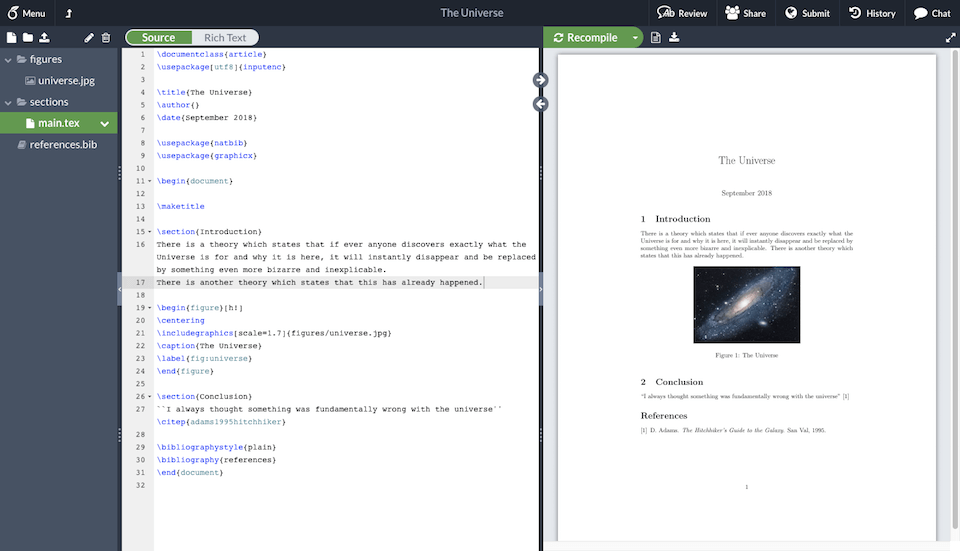
\includegraphics[width=0.6\linewidth]{../intro/overleaf.png}
        \caption{Layout of the Overleaf Online \LaTeX\ Editor.}
    \end{figure}
\end{frame}


\begin{frame}{Installation of \LaTeX}
    Though there are some other distributions of \LaTeX (like Mik\TeX), \TeX Live is recommended in this workshop (or you can use Overleaf instead).

    We recommend beginners to use VS Code as IDE to edit \LaTeX\  files.
    See Hydraallen's \href{https://github.com/Hydraallen/Latex-vscode}{latex-vscode} for installing \TeX Live and \LaTeX\  extension for VS Code.
\end{frame}

\subsection{Documentation}

\begin{frame}[fragile]{Documentation of \LaTeX}

    If you've installed a full version of \TeX Live (as strongly recommended), the full \LaTeX\ documentation is already on your computer. \medskip

    \pause

    Open the command line and input the command

    \begin{minted}{shell}
texdoc <docname>
    \end{minted}

    \pause

    You can also use the online version on \urllink{https://www.latex-project.org/help/documentation/} \medskip

    \pause

    For example, you can use the following types for the \structure{docname}
    \begin{description}
        \item[tex] 		about \structure{\TeX}
        \item[article] 	about documentclass \packagename{article}
        \item[beamer] 	about documentclass \packagename{beamer} (used to create slides)
        \item[pgf]		about packages \packagename{tikz} and \packagename{pgf} (used to draw graphs)
    \end{description}

    \pause

    \smallskip
    Try to \alert{texdoc} about all new things and then you'll be an expert in \LaTeX.
\end{frame}

\subsection*{Starter Pack}

\begin{frame}{Inexperienced \LaTeX\  User Starter Pack}
    \begin{figure}[h]
        \centering
        \includegraphics[width=0.8\textwidth]{../intro/latex_user.png}
    \end{figure}
    \tiny{Frederick Yin, Inexperienced LaTeX User Starter Pack}
\end{frame}

\begin{frame}{Inexperienced \LaTeX\  User Starter Pack 2.0}
    \begin{figure}[h]
        \centering
        \includegraphics[width=0.8\textwidth]{../intro/latex_user_2.png}
    \end{figure}
    \tiny{Frederick Yin, Inexperienced \LaTeX\  Users Starter Pack v2.0}
\end{frame}
